\documentclass{article}

\usepackage{geometry}


%\usepackage{siunitx}
\usepackage{setspace} 
%\doublespacing
\usepackage{cite}
\usepackage{amsmath}
\usepackage{amsthm}
\theoremstyle{remark}
\newtheorem{assumption}{Assumption}
\theoremstyle{remark}
\newtheorem{remark}{Remark}
\theoremstyle{remark}
\newtheorem{theorem}{Theorem}
\theoremstyle{remark}
\newtheorem{lemma}{Lemma}
\theoremstyle{remark}
\newtheorem{property}{Property}
\theoremstyle{remark}
\newtheorem{definition}{Definition}
\usepackage{graphicx}
\usepackage{fancyhdr}
\usepackage[bottom]{footmisc}
%\usepackage{hyperref}
\usepackage{amssymb}
\usepackage{enumerate}
\usepackage[capitalize]{cleveref}
\usepackage[dvipsnames]{xcolor}
%===================================

\newcommand{\marek}[1]{\textcolor{Bittersweet}{#1}}

% Create nicer paragraph spacing
\setlength{\parskip}{2mm plus1mm minus1mm}
\setlength{\parindent}{0cm} 

\title{Optimal Control of An Invasive Plant in n-D Action Space}
%\author{Soheil}

\begin{document}
\maketitle

\section{Problem Definition}
%marek: it is not a good practice to use bolds (much) in research papers
In this research we study the optimal control of \emph{glossy buckthorn}, an invasive plant in the area of New England. The mathematical equation that governs the problem is driven based upon the plant's growing cycle, from when they are seeds to when their fruits are being eaten by other animals, such as birds and rats, and their seeds, again, are being spread to miles away by these animals. In \cref{fig:outline}, the whole process is outlined by details.
% marek: do not include links in pdf files ... not visible when printed
%For more elaborate explanation please refer to \href{https://github.com/rlsquared/gbPopMod}{here}.

\begin{figure}
\centering
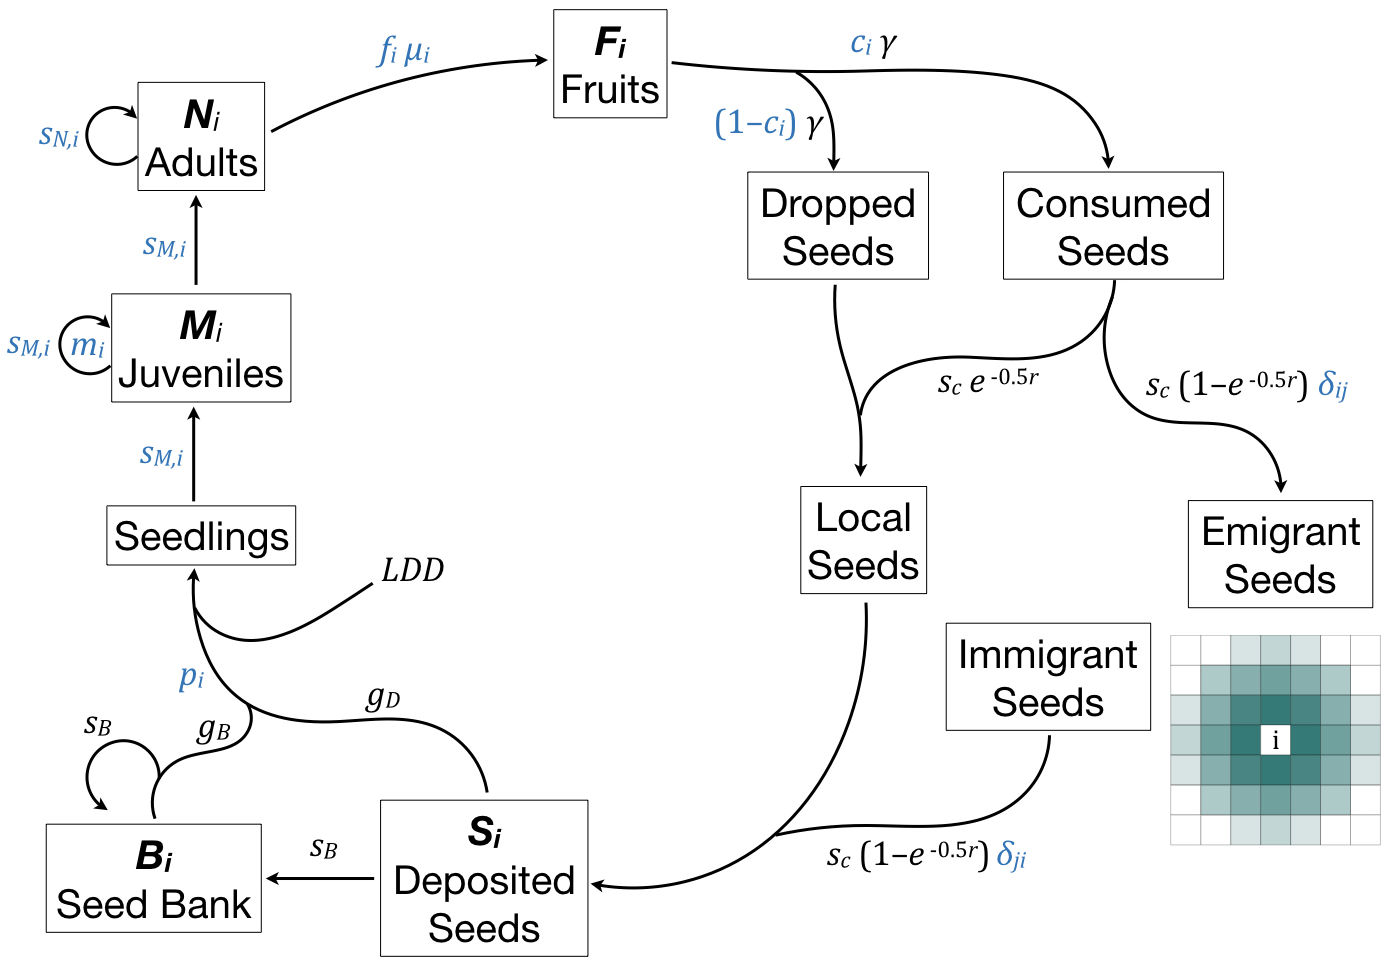
\includegraphics[scale=.2]{model_outline.jpeg}
\caption{The cycle outline} \label{fig:outline}
\end{figure}

We are trying to solve this problem as a Markov decision process. Since, in the first step, we are finding the most basic solution to the problem, we consider the states, actions, rewards, and transition probabilities in its most simplified shape, as follows;

\begin{itemize}
 \item States $\mathcal{S}$: The number of the plant in the whole region, the number of week in a year, the number of other important plans that we might be interested to consider (or possible be affected by the efforts of controlling our plant).
 \item Actions $\mathcal{A}$: Not taking action, spraying pesticide, cutting the plant, growing native competitor plants, spreading mulch, burning the plant
 \item Transition Probabilities $P: \mathcal{S} \times \mathcal{A} \times \mathcal{S}$:
 \item Rewards $r: \mathcal{S} \times \mathcal{A}$: The total net profit of all farmers
\end{itemize}

As mentioned before, we are seeking for the most basic solution for this problem. Therefore, we need to make simplifying assumptions. The following are these assumptions and a number of other considerations we need in our way to tackle the problem;

\begin{enumerate}[(I)]
 \item To reduce the number of states, we only consider the population of the plan in the whole area, as oppose to a state vector consist of the population of the plant in each small grid of the area. This assumption drastically reduces the complexity of the problem.
 \item One possibility for employing different kinds of strategies (taking different actions) is to simply use a threshold in order to apply or to not apply a policy. For instance, pesticide, might or might not be used in a grid of land with a certain area (higher or lower than a threshold).
\end{enumerate}

\section{Related Work}

\subsection{MDPs}

\begin{enumerate}
	\item Bayesian model with a simple state space: \cite{Meisner2016}

	Summary:
	\begin{itemize}
		\item States: At each time point, we classified each field as being in one of three states: low, medium, or high pest density. The exact thresholds for the states were selected so that, aggregated over all eight time points, there was an approximately equal number of observations from each state.
		\item Actions: two different actions: either applying a pesticide or not applying a pesticide
		\item Transition probabilities from state s to state $ s'$ are denoted as $Q_{a,t} (s, s')$; they depend on the action a, time t, origin state s, and destination state s′. Transition probabilities were modeled using a Bayesian ordered logistic regression, so that we could quantify and account for uncertainty in our estimates of these quantities.
		\item costs, $c_{a,t} (s′)$, which depend on the action taken, the time, and the destination state. Both the cost of pesticide application and the cost due to yield loss from L. hesperus damage should be considered. For the cost associated with yield loss due to damage from L. hesperus, we used a hierarchical Bayesian linear mixed model (Gelman and Hill 2009)
		\item Parameter estimation under uncertainty: As both the transition probabilities and yield declines due to L. hesperus are quantities that we had to estimate from the data, there is uncertainty associated with these estimates. To propagate this uncertainty, we obtained, for each time-state combination, 10 000 posterior “samples” of $\sum_{ s' \in S} Q_{a,t}(s,s') [c_{a,t}(s')+V_{t+1}(s')]$ for both possible actions, and selected the action with highest posterior mean as the optimal action. The samples were obtained by considering uncertainty in all three components of the value function: the costs, transition probabilities, and the value function at the next time step.
	
	\end{itemize}
	\item Exploration in very small problems (non-spatial): \cite{Hall2018,Taleghan2015}
	\item Spatial model: \cite{Nicol2017}
	\item \marek{read}: \cite{Albers2018}
	\item \marek{read}: \cite{Mehta2007}
	\item Exponential Population Growth Model in Stan
	\begin{itemize}
		\item We describe here a simple state-space model of population growth and management of an invasive species. The state space is finite, relatively small, and simple. The main challenge is the high level of uncertainty that is involved in the dynamics of the system and in the observations.
		\item Decisions of the policy maker must be based on $y_t$ instead of $N_t$. Note that relying on $y_t$ in place of $N_t$ mildly violates the Markov assumption (Why???).
		\item To be able to run a simulation and study effects of different treatment strategies, we need be able to provide the policy that determines when $z_t=1$. One of the simplest options is a threshold policy: the treatment is applied if and only if the population achieves some specified value threshold.
		\item The policies also need to allow for randomization in order to generate experimental data.

		\begin{equation}
		  \pi(y_t)=\begin{cases}
		    0 & \text{if $y_t <$  threshold}.\\
		    Z & \text{otherwise}.
		  \end{cases}
		\end{equation}
		Z is drawn from a Bernoulli distribution.
		\item



	\end{itemize}
\end{enumerate}

\subsection{One-step (No uncertainty)}

\section{Simple Population-Based Model}


\section{Value Function Approximation}

\section{Linear Value Function Approximation}



\bibliographystyle{plain}
\bibliography{invasive_species}
\end{document}